%% ----------------------------------------------------------------
%% Methods.tex
%% 1113
%% ---------------------------------------------------------------- 
\chapter{Methods} \label{Chapter: Methods}

%Parameters are defined in Results (not in Methods)
%It does not matter if you don't include all the methods, only the ones for the final results.

%Check that you provide enough background information: your reader does not know what you know. Assuming that your reader knows much more than you and therefore omitting background information is a widespread problem with students. A typical example would be a Methods section that directly launches into what you have done without first telling why. Although it is evident to you that to get from A to B you need to do X, this is probably far less obvious to the reader. If you only tell the reader that you did X, she is confused. Why did you do X? Never assume that the reader knows your motivation, or the details of every method you used, or why your research question is relevant. Tell her.

%Plagiarism: use of code (this includes open source code!) that was not written by you, without acknowledgement of the source

%Check that the reader can replicate your results. Verify that your Methods section (and the supplementary sections if any) contains everything that the reader needs to know. Also, check that you provide links to your code and your data if it can be released without violating anyone’s privacy.

%\begin{enumerate}
%\item How am I going to measure it?
%\item How am I going to prove it?
%\end{enumerate}

Most of the computation work is performed on the \textit{IRIDIS High-Performance Computing Facility}, with the help of associated support services at the university. They make use of NVIDIA\textregistered$ $ GeForce GTX 1080 Ti Graphical Processing Units (\textit{GPU}s). The use of the GPUs has been possible thanks to the CUDA 9.0 toolkit\footnote{\url{https://developer.nvidia.com/cuda-toolkit}}.

\section{Dataset}
For this project, the database produced and made public by \cite{Zhou2014} is used\footnote{It can be accessed at \url{https://www.princeton.edu/\~7Ejzthree/datasets/ICML2014/}}. This database has been taken as the flagship benchmark since its release and making use of it allows fair comparisons with most state-of-the-art algorithms. This dataset includes two sub-sets (training and test) of proteins that come from different sources in order to ensure that the test set is composed of completely new samples. For this same reason, they filtered the training set, stripping out every sequence that held 25\% or more similarity with any protein from the test set.
The training set was obtained from PISCES server (\cite{Wang2003})\footnote{\url{http://dunbrack.fccc.edu/Guoli/PISCES\_OptionPage.php}} from a date before January 2014, which was in time culled from the Protein Data Bank (PDB) (\cite{Berman2003}).
It has an original size of 6133 proteins and 5534 after the filtering. The test set comes from the CB513 dataset \cite{Cuff1999} and includes 514 sequences\footnote{Originally 513, but the last one was split in two since it was longer than the 700 amino-acids limit.}.

Protein sequences can be up to 700 amino acids long (with an average of about 214) and have already been pre-processed by \cite{Zhou2014}, with one-hot encoded inputs for the 21 one types of amino-acid along with a 21-long vector of the \textit{pssm} values and their one-hot encoded secondary structure Q8 classes. The appearance frequencies of the eight classes in both datasets are shown in Figure \ref{fig:targetfreq}.

A subset of 256 proteins was taken out of the training set and used for validation, leaving 5278 proteins for the training. This splitting is common in previous papers (\cite{Zhou2014,Sønderby2014,Busia2017,Jurtz2017,Hattori2017}).

\begin{table}[h]
	\centering
	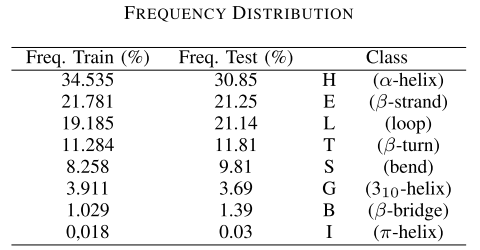
\includegraphics[width=0.5\linewidth]{targetfreq}
	\caption{Target frequencies on the CB6133 (left) and the CB513 (right). Table reproduced from \cite{Hattori2017}.}
	\label{fig:targetfreq}
\end{table}


\section{Network of study}\label{sect:network}

The interpretability methods could be applied to any state-of-the-art network since these would provide the most refined information about the secondary structure problem. However, in order to reach peak accuracies, these models include incredibly huge models that are not handy to work on (especially when it comes to computational time). For this reason, a simpler network is produced and employed for this analysis, with the hope that it will not lose generality over more complex networks.

The network that is used in this study has been built and trained using the open-source code developed by \cite{Jurtz2017}\footnote{Accesible at \url{https://github.com/vanessajurtz/lasagne4bio}.} on the \textit{Lasagne} framework (\cite{Dieleman2015}). While most training configurations are preserved (cross-entropy with L2 regularisation as the error function, batch normalisation, uniform glorot initialisation, mini-batches of size 64, RMSprop rule updates, gradient clipping), the network architecture itself is completely rebuilt. The weights for the final model are the ones from the epoch that has the best performance on the validation set.

The network is composed of three successive convolutional networks and a dense layer on top. Each of the convolutional layers contains three sets of filters of size 3, 5 and 7, respectively, with 16 filters per size. There are skip connections that by-pass every convolutional network in the same fashion as \textit{ResNet}(\cite{He2015}), so the dense layer gets the concatenation of the raw input along with the outputs from the first, second and third layer altogether.
The dense layer has 200 neurons and is connected to a \textit{soft-max} layer that gives the output (secondary structure prediction). The convolution operation is carried out with padding at each end of the sequence to preserve the length of the sequences throughout the convolution operations and produce in the final step one label per position. A sketch of the network can be seen in Figure \ref{fig:pureConv}.

% Check number of weights at the dense layer. Done, they seem alright (186x200)
\begin{figure}
\centering
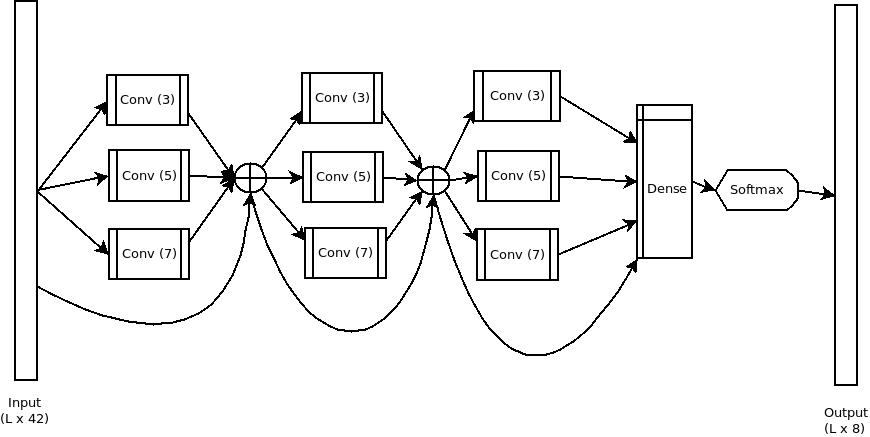
\includegraphics[width=0.8\linewidth]{Figures/pureConv}
\caption{\textit{Schema of network architecture}. There are three convolutional layers with filters of size 3, 5 and 7, followed by a dense layer and the softmax. Skip-connections bring together the output from all previous layers to each new layer.}
\label{fig:pureConv}
\end{figure}


The total window size for this network is 19, meaning that for making a single secondary structure classification the network obtains information from 9 adjacent positions at each side. Although some authors claim that the network should capture long interactions between amino-acids (\cite{Li2016,Lin2016,Hattori2017,Heffernan2017}), it has been proven that most relevant information comes from the local environment (\cite{Busia2017}), so the limited window size should not impinge the model. This fact also supports the idea that the skip connections are beneficial since they avoid the most local information to be ``washed out" in upper layers (\cite{Busia2017}).

% TRy network with a total window size of 43, as Busia did


\section{Feature visualization}
This work only uses first-layer filters as feature visualization means. These only give a very limited amount of information about the very first features created, with a hard interpretation due to the depth of the network. In this case, we have filters with three different sizes to inspect: 3x42, 5x42 and 7x42. They can be visualized in a intuitive way in the form of \textit{sequence logos}, which can be generated with the \textit{Seq2Logo} tool (\cite{Thomsen2012}). Other feature visualisation techniques remain for future work.


\section{Saliency maps} \label{sect:saliency}

% SAliency maps pre or post softmax?

Saliency maps have been calculated by the conventional technique of computing the gradient of the output with respect to the inputs and multiplying it by the value of the input itself (\cite{Shrikumar2016}). A significant difference between this work and most previous papers that make use of saliency maps is that they perform many-to-one classification (one output class per sequence/image), here the classification task is many-to-many (each position of the sequence is assigned a class), producing many saliency maps for a single sequence. More specifically, every single position produces a saliency map that contains the influence of the 42-size input (21 amino-acids plus 21 \textit{pssm} scores) onto the 8-size soft-max output. This information covers the 19 positions surrounding the one being predicted, ending up with a saliency map with total dimension 8x42x19. They are computed using Theano framework (\cite{TheTheanoDevelopmentTeam2016}) since it allows automatic differentiation of symbolical expressions and the use of GPUs.

\subsection{Extracting information from saliency maps}
The presence of overlapping saliency maps allows for different ways of aggregating them and extracting meaningful information. In order to obtain information for a specific sequence, the overlapping saliency maps of such sequence could just be added up, resulting in a single, long \textit{sequence-specific} saliency map of size 8x42x$l$.

By changing the focus to general information of the network behaviour, the sheer addition of all saliency maps produces a single 8x42x19 map with an average behaviour. From this map we could extract information about the general behaviour of a particular class (\textit{class-specific} saliency map) or a certain amino-acid (\textit{pssm-specific} saliency map). If a more fine-grained inspection is desired, clustering techniques can be used, and every cluster creates their independent 8x42x19 representative map by addition of all their components.

%Problems with saliency aggregation %INclude my plots with the sliding saliencies
%On the right, saliencies of subsequent single positions. Each line of a plot represents one amino acid. Each plot corresponds to one position. X axis is the window size (19)

%Motifs slide through the saliencies, which makes:
%Sheer aggregation to capture the sliding effect
%Clustering of full saliencies useless 

%Solution:
%By aggregating each saliency on its window length (right), the motifs are preserved %INclude my plots with the sliding window aggregations
%Clustering on the saliencies (cosine) in the positions with a high prediction for one class can show different kinds of motifs that activate that class

%\subsection{Clustering on saliencies}
%Using the per-class window-aggregated version of individual saliency maps (4 dimensions left)
%Cosine distance metric.
%Show either all profiles per-cluster (3 dimensions) or aggregated profiles (2 dimensions)

\section{Open-source}

As it is the standard practice in both the bioinformatics and machine learning research communities, all the code from this project has been released as open-source in the web platform GitHub and can be accessed through the URL \url{https://github.com/Juillermo/lasagne4bio}, with the hope that the tools here developed can be of use for future research.
